\documentclass[]{beamer}

% !TeX program = lualatex
\usepackage{pacchetti-slides}

%%%%%%%%%%%%%%%%%%%%%%%%%%%%%%%%%%%%%%% COLORI

\definecolor{turquoise}{RGB}{0, 247, 230}
\definecolor{goldenyellow}{RGB}{255, 218, 66}
\definecolor{fuchsia}{RGB}{255, 0, 172}
\definecolor{electric-blue}{RGB}{55, 0, 255}

\definecolor{blond}{RGB}{251,231,161}
\definecolor{skincolor}{RGB}{224,177,132}
\definecolor{idea}{RGB}{254,231,2} 	        %giallo ideee

%%%%%%%%%%%%%%%%%%%%%%%%%%%%%%%%%%%%%%% HEAD COMMANDS	
\newcommand{\inghead}{% 
	\textcolor{darkturquoise}{\LARGE\textbf{Ingredienti}\ }
}

\newcommand{\mathead}{% 
	\textcolor{darkturquoise}{\LARGE\textbf{Materiale utile}\ }
}
\newcommand{\prephead}{% 
	\textcolor{fuchsiapink}{\LARGE\textbf{Preparazione}\ } }
\newcommand{\hinthead}{% 
	\textcolor{cerisepink}{\huge{Tip:}}
}

%%%%%%%%%%%%%%%%%%%%%%%%%%%%%%%%%%%%%% Math commands

% Comandi per i teoremi, definizioni ed esmpi
\theoremstyle{plain}
\newtheorem{thm}{Teorema} % reset theorem numbering for each chapter
\newtheorem{post}{Postulato} % reset theorem numbering for each chapter
\newtheorem{lem}{Lemma}

\theoremstyle{definition}
\newtheorem{defn}{Definizione} % definition numbers are dependent on theorem numbers
\newtheorem{exmp}{Esempio} % same for example numbers
\newtheorem*{ach}{Attenzione!}

% Shortcut
\newcommand{\SigmaX}{\hat{\sigma}^{(x)}}
\newcommand{\SigmaY}{\hat{\sigma}^{(y)}}
\newcommand{\SigmaZ}{\hat{\sigma}^{(z)}}

\newcommand{\Hilb}{\mathcal{H}}
\newcommand{\Id}{\hat{\mathcal{I}}}
\newcommand{\LinSet}{\mathscr{L}}
\newcommand{\ChoiState}[1]{\hat{\rho}_\text{CJ}^{#1}}

\DeclareMathOperator{\Tr}{tr}

\newcommand{\VerticalBrace}[4][]{%
	% #1 = draw options
	% #2 = top mark
	% #2 = bottom mark
	% #4 = label
	\begin{tikzpicture}[overlay,remember picture]
	\tikzmath{coordinate \p,\q;\p=(pic cs:#2);\q=(pic cs:#3);\maxx=max(\px,\qx);}
	\draw[xshift=1ex,decorate,decoration={brace, amplitude=1.5ex}, #1] 
	([yshift=1.5ex]{{pic cs:#2} -| \maxx pt,0})  -- ([yshift=-.5ex]{{pic cs:#3} -| \maxx pt,0})
	node[My Node Style] {#4};
	\end{tikzpicture}
}


%box carini
\newenvironment<>{ideablock}[1]{%
	\setbeamercolor{block title}{fg=white,bg=fuchsia}%
	\begin{block}#2{#1}}{\end{block}}

\newenvironment<>{defblock}[1]{%
	\setbeamercolor{block title}{fg=white,bg=goldenyellow}%
	\begin{block}#2{#1}}{\end{block}}

\newenvironment<>{theoblock}[1]{%
	\setbeamercolor{block title}{fg=white,bg=turquoise!80!black}%
	\begin{block}#2{#1}}{\end{block}}


% due nuovi comandi per allineare le cose bene
\newcommand\parallelcontent[2]{
	\begin{columns}[t]
		\column{0.5\textwidth} #1
		\column{0.5\textwidth} #2
	\end{columns}
}
\newcommand\parallelitem[2]{
	\parallelcontent
	{\begin{itemize} \item #1 \end{itemize}}
	{\begin{itemize} \item #2 \end{itemize}}
}

%Citazioni
\newcommand{\easycite}[2]{
	[\textcolor{electric-blue}{#1 - #2}]
}

%%%%%%%%%%%%%%%%%%%%%%%%%%%%%%%%%%%%%%% MATH SYMBOLS
\newcommand{\R}{{\mathbb{R}}}
\newcommand{\N}{{\mathbb{N}}}

 \newcommand{\pprec}{\prec\mathrel{\mkern-5mu}\prec}

% % Bibliografia
% \usepackage[backend=bibtex,doi=false,isbn=false,url=false]{biblatex}
\usepackage[backend=bibtex, style=authoryear]{biblatex}
% Authors in small caps in citation and bibliography
% \renewcommand*{\mkbibnamelast}[1]{\textsc{#1}}
% \renewcommand*{\mkbibnameprefix}[1]{\textsc{#1}}
\addbibresource{bibliografia.bib}

% \setbeameroption{show notes on second screen=bottom}

\usetheme{PaloAlto}
\setbeamercovered{transparent} %per rendere sbiadito cio' che verra'
\setbeamertemplate{navigation symbols}{}

\usecolortheme{rose} 
\setbeamercolor{structure}{fg=turquoise!70!black}


%Information to be included in the title page:
\title[Generalisation of BH Area theorem]
{A generalisation of the Black Hole Area theorem with Index form methods}

\institute[UniPi]{
\includegraphics[height=2.5cm]{Immagini/LogoUniPi/marchio_unipi_pant541.pdf}}

\author[Veronica Sacchi]{\textit{Candidate}: Veronica Sacchi \hfill\textit{Supervisor}: E.A. Kontou}  

\logo{
\includegraphics[height=1.4cm]{Immagini/LogoUniPi/cherubino_white.pdf}}
\date[16-09-2022]{16th September 2022}

\begin{document}

	\usebackgroundtemplate{
		\adjustbox{height=0.8\paperheight, , raise=-9cm, right=15cm}{
			\transparent{0.05}
			\includegraphics{Immagini/LogoUniPi/cherubino_pant541-eps-converted-to.pdf}
		}
	}

	\begin{frame}
	\titlepage
	\end{frame}
	%%%%%%%%%%%%%%%%%%%%%%%%%%%%%%%%%%%%%%%%%%%%%%%%%%%%%%%%%%%%%%
	\section{Introduction}
	\begin{frame}
		\frametitle{What will we see?}
		\tableofcontents
	\end{frame}
	%%%%%%%%%%%%%%%%%%%%%%%%%%%%%%%%%%%%%%%%%%%%%%%%%%%%%%%%%%%%%%
	\begin{frame}
		\frametitle{The 2020 Nobel Prize}
		\begin{columns}
			\column{0.52\textwidth}
			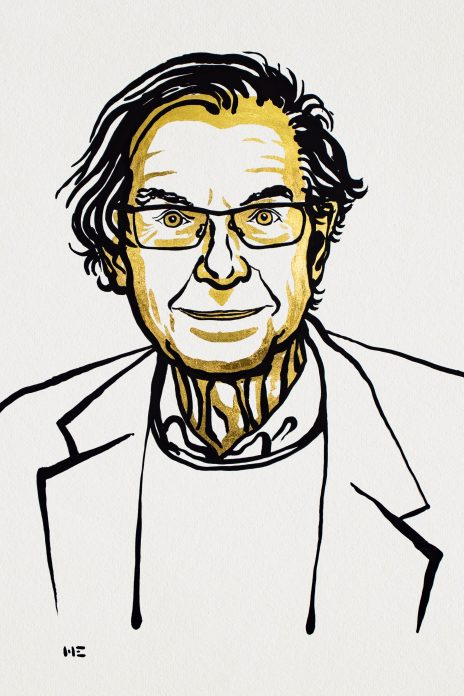
\includegraphics[scale=0.39]{Immagini/Penrose-nobel.jpg}
			\column{0.48\textwidth}
			\centering
			``\emph{For the discovery that black hole formation is a robust prediction of the general theory of relativity.}''
			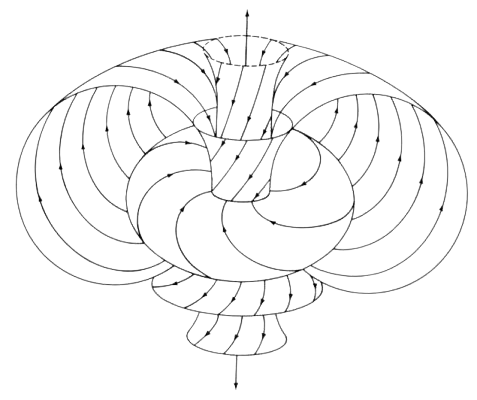
\includegraphics[scale=0.62]{Immagini/twistor-removebg-preview.png}
			\note[item]{Black hole are compact objects light cannot escape from.}
			\note[item]{First black hole solutions: Schwarzschild. Singularity formation possibly due to very high degree of symmetry.}
			\note[item]{Year of Singularity Theorem: 1965}
		\end{columns}
	\end{frame}
	%%%%%%%%%%%%%%%%%%%%%%%%%%%%%%%%%%%%%%%%%%%%%%%%%%%%%%%%%%%%%%
	\begin{frame}
		\frametitle{The Black Hole Area theorem}
		\begin{columns}
			\column{0.6\textwidth}
			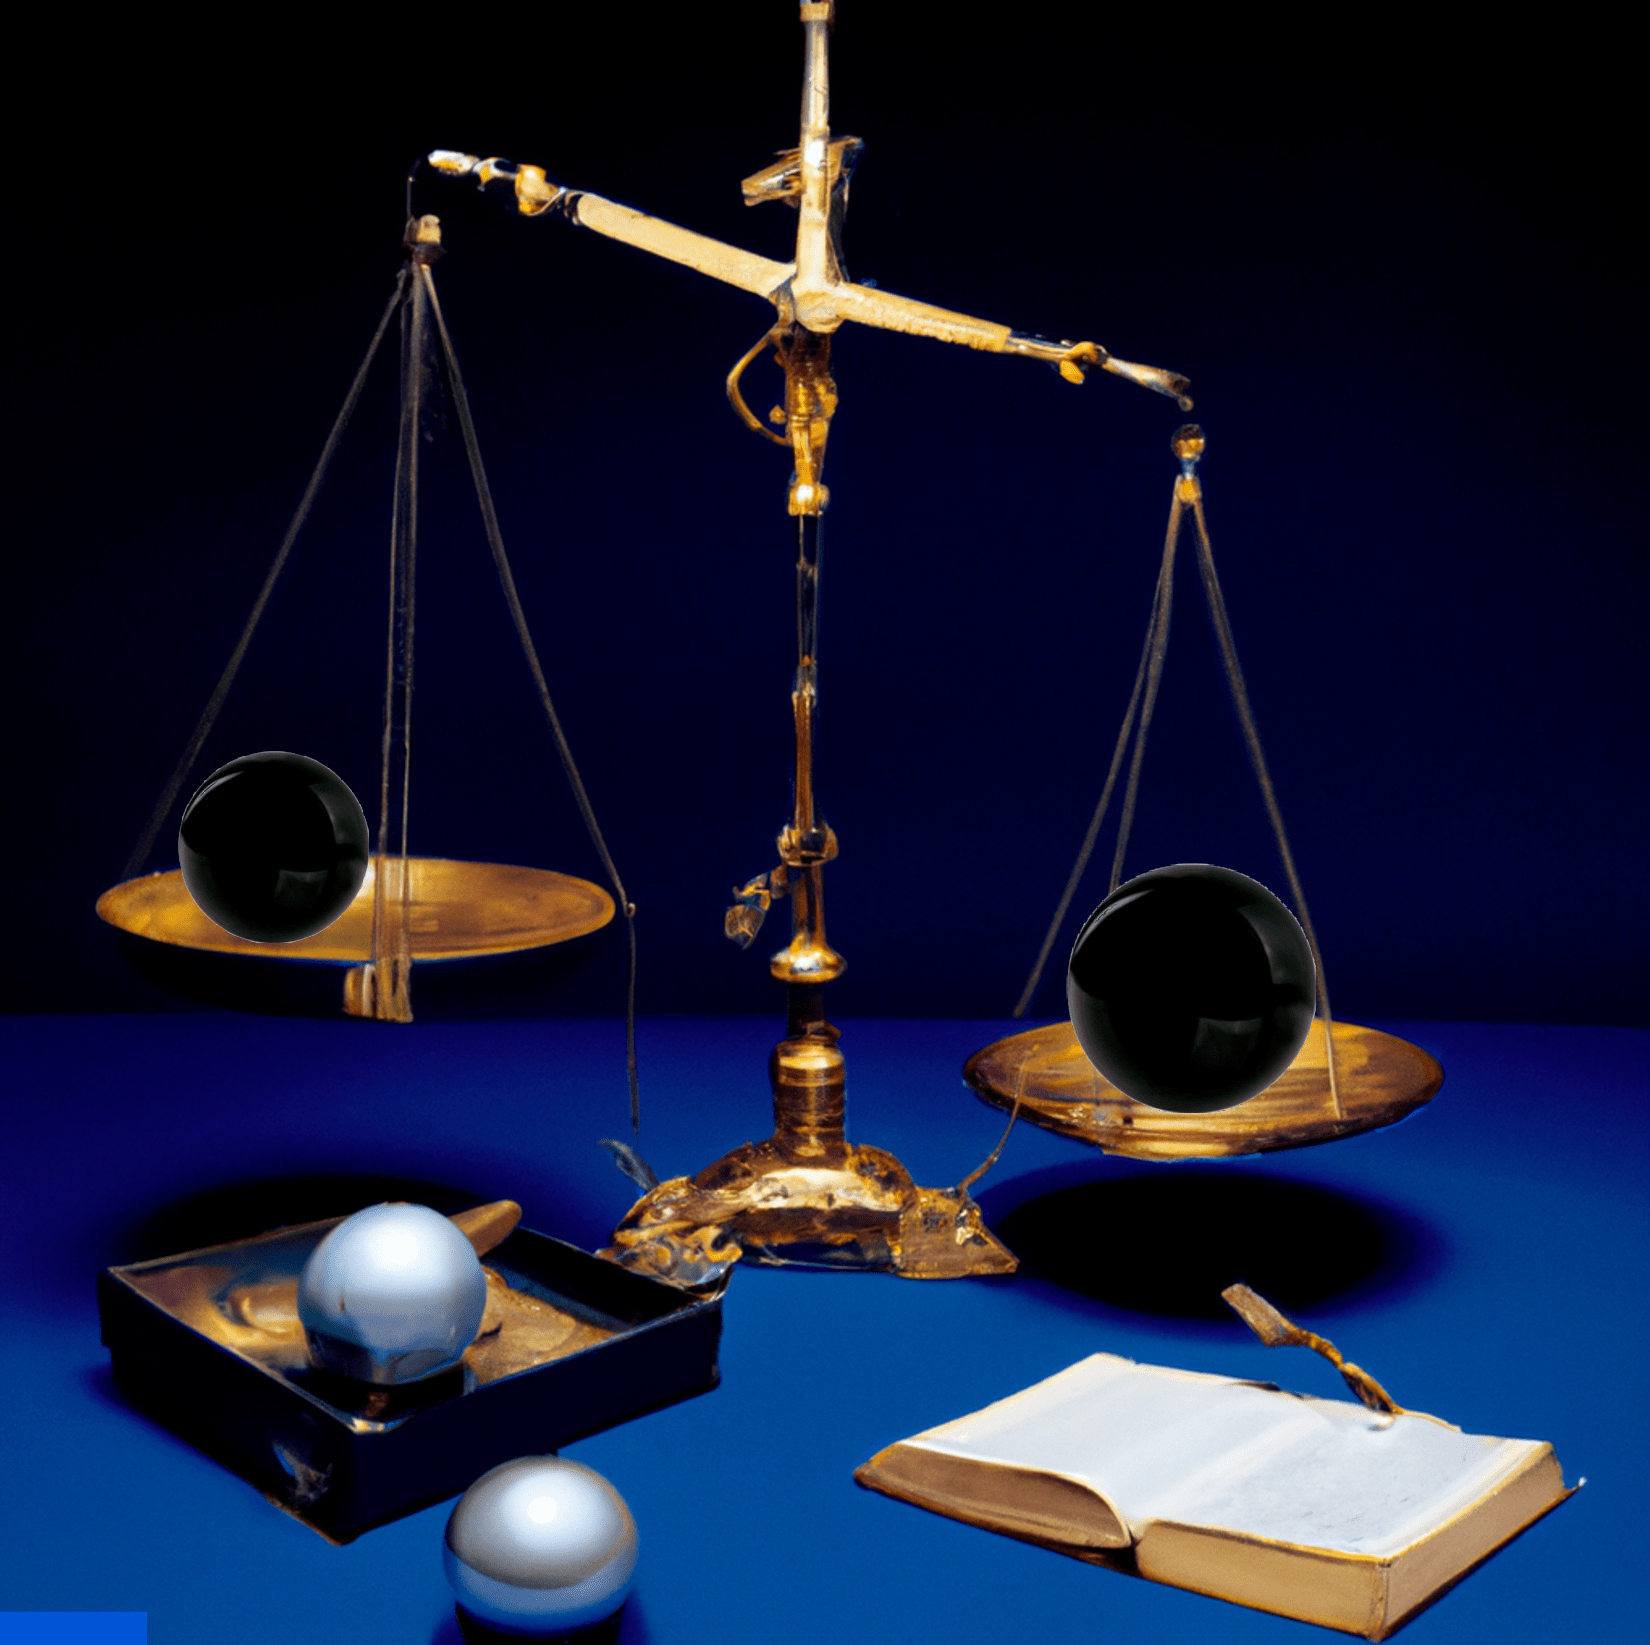
\includegraphics[scale=0.11]{Immagini/DALLE-bh-area.png}
			\column{0.4\textwidth}
			\centering
			[\cite[]{hawking1972black}]
			\[
			\begin{cases}
				\text{Causality}\\
				\text{Energy condition}
			\end{cases}	
			\]
			\[
			\Big\Downarrow	
			\]
			\[
			\delta \mathcal{A}_H \ge 0	
			\]
		\end{columns}
	\note[item]{Extremely general, no simmetry required}
	\note[item]{One of the last relativity theorem: marks the end of the golden age of those theorems.}
	\end{frame}
	%%%%%%%%%%%%%%%%%%%%%%%%%%%%%%%%%%%%%%%%%%%%%%%%%%%%%%%%%%%%%%
	\begin{frame}
		\frametitle{The discovery of Gravitational Waves}
		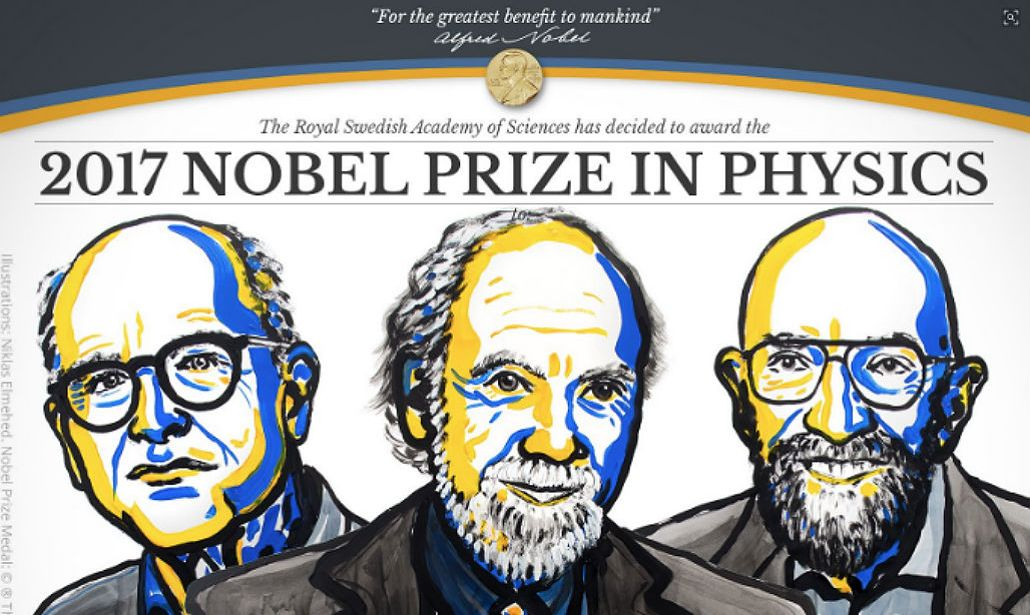
\includegraphics[scale=0.28]{Immagini/2017_Physics_Nobel_full.jpg}
		\note[item]{Finally a way to explore gravity and access to black holes phenomenas}
		\note[item]{Nobel awarded to Rainer Weiss, Barry Barish and Kip Thorne.}
		\note[item]{Ligo detection of 14th September 2015}
		\note[item]{Black Holes were 1.4 billions light years away}
	\end{frame}
	%%%%%%%%%%%%%%%%%%%%%%%%%%%%%%%%%%%%%%%%%%%%%%%%%%%%%%%%%%%%%%
	\begin{frame}
		\frametitle{Observational Evidence of the Area theorem}
		\begin{columns}
			\column{0.6\textwidth}
			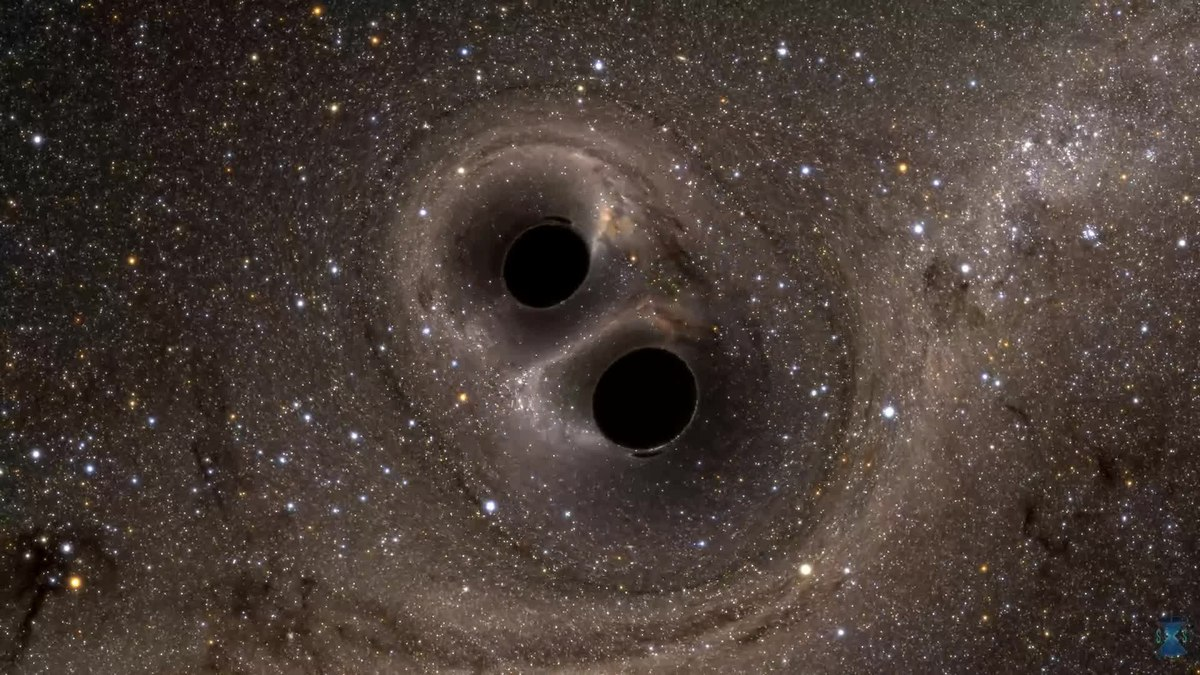
\includegraphics[scale=0.14]{Immagini/BBH_gravitational_lensing_of_gw150914.webm.jpg}
			\column{0.4\textwidth}
			In 2021 physicists from the MIT were able to confirm Hawking's Area theorem with \(95\%\) of confidence. [\cite[]{PhysRevLett.127.011103}].
		\end{columns}
		
		\begin{columns}
			\column{0.47\textwidth}
			M. Isi \emph{et al.} analyse pre- and post-merger data of the event GW150914 in order to measure the mass of the black holes before and after the collision.
			\column{0.53\textwidth}
			\centering
			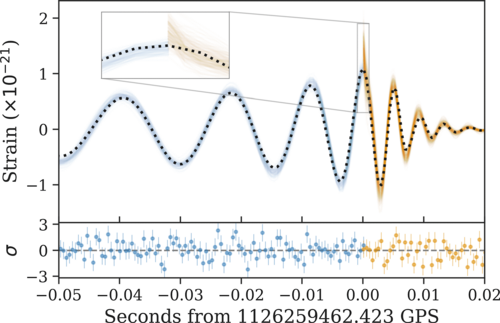
\includegraphics[scale=0.3]{Immagini/medium.png}
		\end{columns}
	\end{frame}
	%%%%%%%%%%%%%%%%%%%%%%%%%%%%%%%%%%%%%%%%%%%%%%%%%%%%%%%%%%%%%%
	\begin{frame}
		\frametitle{Hawking radiation}
		\begin{columns}
			\column{0.6\textwidth}
			\includegraphics[scale=0.5]{Immagini/bh-life-cycle/bh-life-cycle.pdf}
			\column{0.4\textwidth}
			\centering
			\vskip -5pt
			\begin{ideablock}{Non-stationary spacetime}
				\centering
				Alice and Bob don't share a common notion of time.
			\end{ideablock}
			\vskip -17pt
			\[
			\Big\Downarrow
			\]
			Fock spaces connected by a Bogoliubov transformation.
			\[
			\Big\Downarrow
			\]
			\vskip -7pt
			What is vacuum for Bob contains radiation for Alice.
		\end{columns}
	\end{frame}
	%%%%%%%%%%%%%%%%%%%%%%%%%%%%%%%%%%%%%%%%%%%%%%%%%%%%%%%%%%%%%%
	\begin{frame}
		\frametitle{Evaporation Rate}
		\begin{defblock}{Hawking temperature}
			Hawking radiation is distributed with a Planck spectrum of temperature [\cite[]{hawking1975particle}]
			\[
				T_H = \frac{\hbar c^3}{8\pi Gk_B}\cdot \frac{1}{M}.
			\]
		\end{defblock}
		\vskip 10pt
		\begin{columns}
			\column{0.45\textwidth}
			\centering
			Planck spectrum
			\[
				P(\omega) = \frac{\hbar\omega}{e^{8\pi M\omega} - 1}
			\]
			\column{0.1\textwidth}
			\[
			\implies	
			\]
			\column{0.45\textwidth}
			\centering
			``Stefan-Boltzmann Law''
			\[
			\frac{dE}{dt} \propto T_H^4	
			\]
		\end{columns}
		\vskip 10pt
		\begin{theoblock}{Evaporation rate}
			\[
			R_{ev} = -\frac{1}{M}\frac{dM}{dt} \propto T_H^3	
			\]
		\end{theoblock}
	\end{frame}
	%%%%%%%%%%%%%%%%%%%%%%%%%%%%%%%%%%%%%%%%%%%%%%%%%%%%%%%%%%%%%%
	\begin{frame}
		\frametitle{The Classical Black Hole Area theorem}
		\begin{columns}
			\column{0.33\textwidth}
			\centering
			``\emph{The area of the Black Hole Horizon cannot decrease in time.}''
			\vskip 15pt
			% \begin{tikzpicture}
			% 	\node[graduate, stripes=turquoise!80!black, minimum size = 0.5cm] (A) at (0,0){};
			% 	\drawfill[black] (0.5, 0.7) circle (0.3cm);
			% \end{tikzpicture}
			\includegraphics[scale=0.7]{Immagini/classical-bh-area/classical-bh-area.pdf}
			\column{0.27\textwidth}
			\centering
			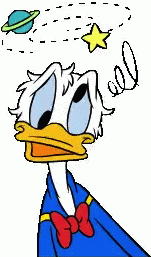
\includegraphics[scale=0.5]{Immagini/donald-duck.png}
			\column{0.39\textwidth}
			\centering
			\includegraphics[scale=0.2]{Immagini/bh-evaporation/bh-evaporation.pdf}
			``\emph{Black Holes evaporate!}''
		\end{columns}
	\end{frame}
	%%%%%%%%%%%%%%%%%%%%%%%%%%%%%%%%%%%%%%%%%%%%%%%%%%%%%%%%%%%%%%
	\section{Energy Conditions}
	\begin{frame}
		\frametitle{Energy Conditions}
		\begin{defblock}{What is an energy condition?}
			It is a condition on a contraction of the stress energy tensor.

			E.g. NEC: \(T_{\mu\nu}U^{\mu}U^{\nu} \ge 0\)  \(\forall U\) null vectors.
		\end{defblock}
			\begin{itemize}
				\item \(R_{\mu\nu} - \frac{1}{2}Rg_{\mu\nu} = \frac{8\pi G}{c^4} T_{\mu\nu}\).
				\item Perfect fluid: \(\rho + p \ge 0\).
				\item Rule out pathological solutions of Einstein equations.
				\item Express ``attractiveness of gravity".
			\end{itemize}
		\vskip 10 pt 
		\begin{center}
			\textbf{BUT}
		\end{center}
		\begin{ideablock}{}
			\centering
			All \emph{pointwise} energy conditions will be violated by quantum fields. [\cite{epstein1965nonpositivity}]
		\end{ideablock}
	\end{frame}
	%%%%%%%%%%%%%%%%%%%%%%%%%%%%%%%%%%%%%%%%%%%%%%%%%%%%%%%%%%%%%%
	\begin{frame}
		\frametitle{Averaged Energy Conditions}
		\begin{columns}
			\column{0.43\textwidth}
			\begin{ideablock}{\emoji{light-bulb} Quantum interest \emoji{light-bulb} } 
				\centering
				Local violations are often overcompensated for in other regions of spacetime.
			\end{ideablock}
			\column{0.57\textwidth}
			\includegraphics[scale=0.5]{Immagini/averaged-conditions/averaged-conditions.pdf}
		\end{columns}
		\[
			\Big\Downarrow
		\]
		\centering
		\[
			R_{\mu\nu} - \frac{1}{2}Rg_{\mu\nu} = \frac{8\pi G}{c^4} \langle T_{\mu\nu} \rangle
		\]
		\begin{defblock}{ANEC}
			\[
				\int_{\gamma} \langle T_{\mu\nu}\rangle U^{\mu}U^{\nu} d\lambda \ge 0 \dashrightarrow \int_{\gamma}  R_{\mu\nu}U^{\mu}U^{\nu} d\lambda \ge 0
			\]
		\end{defblock}
		% \textbf{Problems}
		% \begin{itemize}
		% 	\item Often either too weak to prove a singularity theorem, or too strong to be proven by QFT.
		% 	\item No clear physical interpretation.
		% \end{itemize}
	\end{frame}
	%%%%%%%%%%%%%%%%%%%%%%%%%%%%%%%%%%%%%%%%%%%%%%%%%%%%%%%%%%%%%%
	\section{Index form methods}
	\subsection{Focal points\ldots}
	\begin{frame}
		\frametitle{Focal Points\ldots}
		\begin{columns}
			\column{0.65\textwidth}
			\centering
			\includegraphics[scale=1.2]{Immagini/focal-points/focal-points.pdf}
			\column{0.35\textwidth}
			\begin{defblock}{Focal Points}
				Let \(\gamma\) be a geodesic \(\perp P\).
				
				\(\gamma(r)\), where \(r \neq 0\), is a \emph{focal point} of \(P\) along \(\gamma\) if:
				\begin{itemize}
					\item \(\exists V\neq 0\) \(P\)-Jacobi field on \(\gamma\).
					\item \(V(r) = 0\).
				\end{itemize}
			\end{defblock}
		\end{columns}
	\end{frame}
	%%%%%%%%%%%%%%%%%%%%%%%%%%%%%%%%%%%%%%%%%%%%%%%%%%%%%%%%%%%%%%
	\begin{frame}
		\frametitle{Focal Points\ldots}
		\begin{ideablock}{Why are focal points important?}
			\centering
			Past a focal point a timelike geodesic is not length-extremizing anymore!
		\end{ideablock}
		\begin{columns}
			\column{0.5\textwidth}
			\centering
			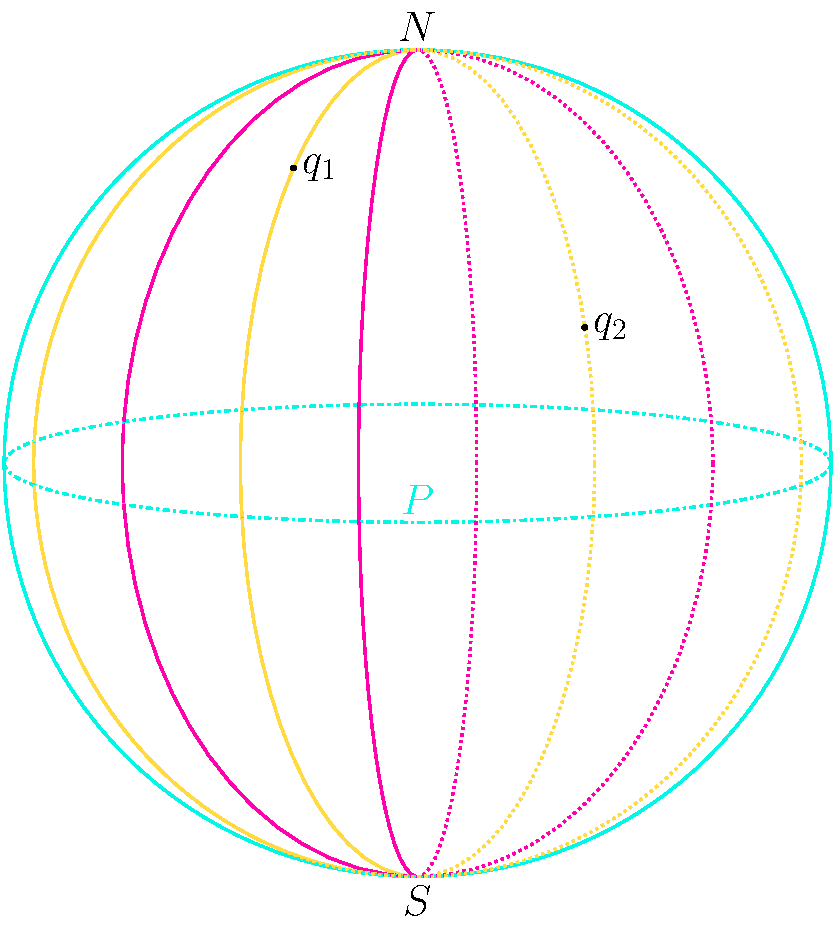
\includegraphics[scale=0.33]{Immagini/sphere-focal-points/sphere-focal-points.pdf}
			\column{0.5\textwidth}
			\begin{defblock}{Promptness}
				\(\gamma\) from \(P\) to \(q\) is \emph{prompt} if there is no causal path from \(P\) to any point \(q'\) in the past of \(q\). [\cite[]{witten2020light}]
			\end{defblock}
		\end{columns}
	\end{frame}
	%%%%%%%%%%%%%%%%%%%%%%%%%%%%%%%%%%%%%%%%%%%%%%%%%%%%%%%%%%%%%%
	\subsection{\ldots and where to find them}
	\begin{frame}
		\frametitle{The Raychaudhuri's equation}
		\begin{defblock}{The expansion}
			\(\theta\) is the variation of the transverse area of a congruence of geodesics.
			\[
			\theta = \nabla_{\mu}U^{\mu}	
			\]
		\end{defblock}
		\vskip 10pt
		\begin{columns}
			\column{0.45\textwidth}
			\centering
				\includegraphics[scale=0.7]{Immagini/raychaudhuri/focal-points.pdf}
			\column{0.55\textwidth}
			\[
				\frac{D}{D\lambda}\theta \le -\frac{\theta^2}{d - 2} - R_{\mu\nu}U^{\mu}U^{\nu}
			\]
			\vskip 10pt
			\begin{ideablock}{Existence criterion for focal points}
				\centering
				\(\vert\theta\vert \rightarrow +\infty \implies \) 
				a focal point is developed.
			\end{ideablock}
			% \begin{align*}
			% 	\frac{D}{D\lambda}\theta &= -\frac{\theta^2}{d - 2} - \sigma_{\mu\nu}\sigma^{\mu\nu} + \omega_{\mu\nu}\omega^{\mu\nu}  - R_{\mu\nu}U^{\mu}U^{\nu} \\
			% 	&\le -\frac{\theta^2}{d - 2} - R_{\mu\nu}U^{\mu}U^{\nu}
			% \end{align*}
		\end{columns}
	\end{frame}
	%%%%%%%%%%%%%%%%%%%%%%%%%%%%%%%%%%%%%%%%%%%%%%%%%%%%%%%%%%%%%%
	\subsection{The Index form method}
	\begin{frame}
		\frametitle{\ldots and where to find them}
		For null geodesics we study the \emph{energy} or \emph{action} functional:
		\[
			E[\gamma] \coloneqq \frac{1}{2}\int_{0}^{l} g(\gamma'(\lambda), \gamma'(\lambda))d\lambda	
		\]
		\begin{ideablock}{Index form method}
			\centering
			No focal points \(\implies \textbf{H}(V) \equiv\frac{d^2E[\gamma_s]}{ds^2}\Big\vert_{s = 0} < 0\)
		\end{ideablock}
	
		\begin{theoblock}{Existence criterion for focal points}
			If there exists \(f(\lambda)\) such that \(f(0) = 1\), \(f(\ell) = 0\) and
			\[
				\int_{0}^{\ell} \big((n -2)(\nabla_Uf)^2 - f^2R_{\mu\nu}U^{\mu}U^{\nu} \big)(\lambda) d\lambda\le -(n-2)U_{\mu}\mathrm{H}^{\mu}\Big\vert_{\lambda = 0}	
			\]
			then \(\gamma\) contains a focal point to \(P\) before \(\ell\)
		\end{theoblock}
	\end{frame}
	%%%%%%%%%%%%%%%%%%%%%%%%%%%%%%%%%%%%%%%%%%%%%%%%%%%%%%%%%%%%%%
	\begin{frame}
		\frametitle{The mean normal curvature}
		\begin{columns}
			\column{0.43\textwidth}
			\centering
			\begin{ideablock}{Area variation}
				\[
				\delta_{U}\mathcal{A}_P = \int_{P} \mathrm{H}^{\mu}U_{\mu}.
				\]	
			\end{ideablock}
			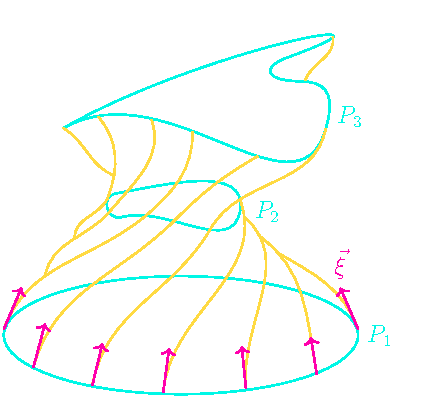
\includegraphics[scale=0.66]{Immagini/area-and-curvature/area-and-curvature.pdf}
			\column{0.57\textwidth}
			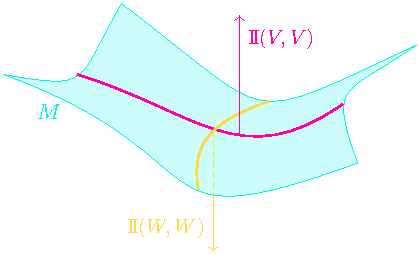
\includegraphics[scale=0.8]{Immagini/shape-tensor/shape-tensor.pdf}
			\begin{defblock}{Mean normal curvature}
				\[
				\mathrm{H}^{\mu}(p) = \frac{1}{n} \sum_{i=1}^{n} \epsilon_i \mathrm{I\!I}^{\mu}(\textbf{e}_i, \textbf{e}_i).
				\]
				\end{defblock}
		\end{columns}
	\end{frame}
	%%%%%%%%%%%%%%%%%%%%%%%%%%%%%%%%%%%%%%%%%%%%%%%%%%%%%%%%%%%%%%
	\section{The Black Hole Area Theorem}
	\subsection{The classical area theorem}
	\begin{frame}
		\frametitle{The Classical Black Hole Area Theorem}

		\begin{columns}
			\column{0.4\textwidth}
			\centering
			\begin{itemize}
				\item \emph{Causal black hole region} \(B\): \(B \coloneqq M \setminus J^-(\mathscr{I}^+)\).
				\item \emph{Causal event horizion} \(H\): \(H\coloneqq \partial J^-(\mathscr{I}^+) \cap M \).
			\end{itemize}	
			\includegraphics[scale=0.15]{Immagini/black-holes/black-holes.pdf}
			\column{0.6\textwidth}
			\begin{theoblock}{Hawking's Area Theorem}
				Let \((M, g_{\mu\nu})\) such that:
				\begin{itemize}
					\item SAP;
					\item \(R_{\mu\nu}U^{\mu}U^{\nu} \ge 0\).
				\end{itemize} 
				
				Given two subsequent ``snapshots'' of the horizion \(H\)
				\[
				\mathscr{H}_1 = H \cap \Sigma_1 \quad \quad \mathscr{H}_2 = H \cap \Sigma_2,
				\]
				the area of \(\mathscr{H}_2\) is greater or equal than the area of \(\mathscr{H}_1\).
			\end{theoblock}
			\begin{ideablock}{}
				\[
					\delta \mathcal{A} \ge 0.
				\]
			\end{ideablock}
		\end{columns}
	\end{frame}
	%%%%%%%%%%%%%%%%%%%%%%%%%%%%%%%%%%%%%%%%%%%%%%%%%%%%%%%%%%%%%%
	\subsection{A generalisation of the theorem}
	\begin{frame}
		\frametitle{The Generalised Black Hole Area Theorem}
		
		\begin{columns}
			\column{0.55\textwidth}
			% \centering
			\begin{align*}
				J_{\ell}[f]\coloneqq & \int_{0}^{\ell} \big((n -2)(\nabla_Uf)^2 \\
				& - f^2R_{\mu\nu}U^{\mu}U^{\nu} \big)d\lambda
			\end{align*}
			\vskip -20pt
			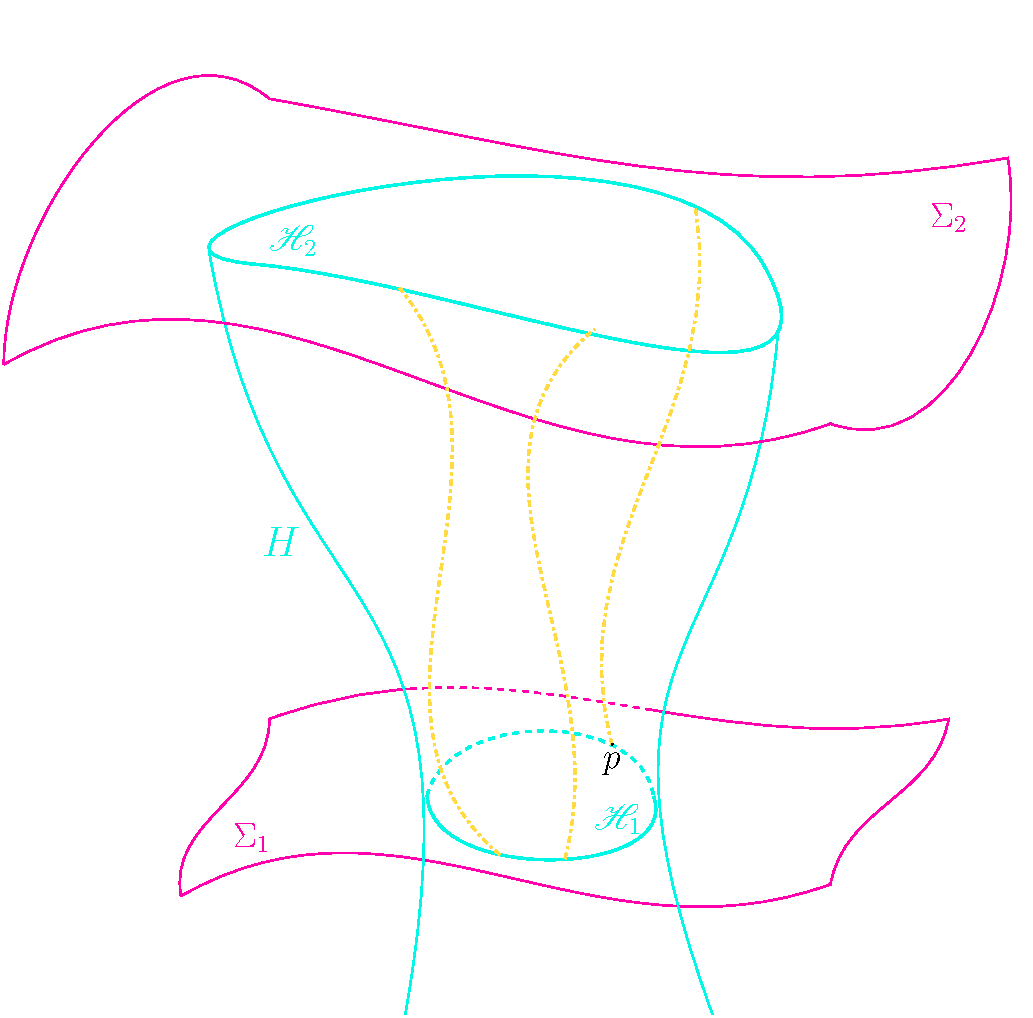
\includegraphics[scale=0.33]{Immagini/flow-generators/flow-generators.pdf}
			\column{0.45\textwidth}
			\vskip -11pt
			\begin{theoblock}{The Generalised Area Theorem}
				Let \((M, g_{\mu\nu})\) SAP and \(\mathscr{H} = H \cap \Sigma\) as before. Then on its horizon
				\begin{align*}
					U_{\mu}\mathrm{H}^{\mu}(p) \ge &-\frac{1}{n - 2} \cdot \\
					&\cdot\inf_{\substack{f\in C^{\infty}_{1,0}[0, \ell]\\ \ell > 0}}J_{\ell}[f]\\
					&\coloneqq -\frac{\mathcal{V}}{n - 2}
				\end{align*}
			\end{theoblock}
			\begin{ideablock}{}
				\[
					\delta \mathcal{A} \ge -\frac{\mathcal{V}}{n - 2}.
				\]
			\end{ideablock}
		\end{columns}
	\end{frame}
	%%%%%%%%%%%%%%%%%%%%%%%%%%%%%%%%%%%%%%%%%%%%%%%%%%%%%%%%%%%%%%
	\begin{frame}{A proof of the Generalised Area theorem}
		\vskip -11pt
		\[
			U_{\mu}\mathrm{H}^{\mu}(p') < -\frac{1}{n - 2}\underbrace{\int_{0}^{\ell} \big((n -2)(\nabla_Uf)^2 - f^2R_{\mu\nu}U^{\mu}U^{\nu} \big) d\lambda}_{J_{\ell}[f]}
		\]
		\vskip -14pt
		\begin{columns}
			\column{0.6\textwidth}
			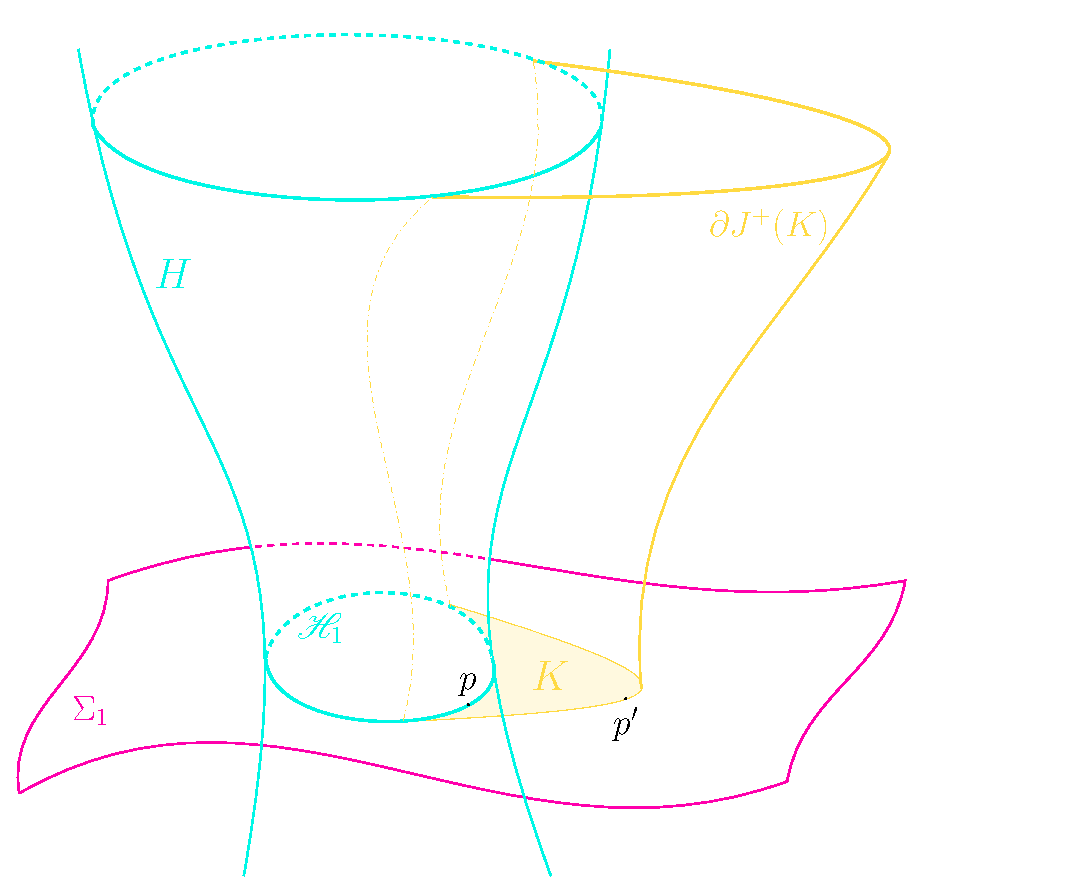
\includegraphics[scale=0.4]{Immagini/extension-area-theorem/extension-area-theorem.pdf}
			\column{0.4\textwidth}
			\centering
			\vskip -15pt
			\[
			\Big\Downarrow	
			\]
			\(\exists\) a focal point on \(\partial J^+(K)\)
			\vskip 5pt
			\pause
			\begin{tikzpicture}[scale=0.5]
				\foreach \i in {0, 1,..., 7}{
					\begin{scope}[shift={(\i, 0)}, rotate=0]
					\draw[thick, fuchsia] (0, -0.25) -- (0.5, 0.25) -- (1, -0.25);
					\end{scope}
				}
			\end{tikzpicture}
			\vskip 5pt
			\(\partial J^+(K)\) is foliated by prompt curves
			\vskip -17pt
			\[
			\Big \Uparrow	
			\]
			\vskip -3pt
			Causality

		\end{columns}
	\end{frame}
	%%%%%%%%%%%%%%%%%%%%%%%%%%%%%%%%%%%%%%%%%%%%%%%%%%%%%%%%%%%%%%
	\begin{frame}
		\frametitle{Classical Energy conditions}
		\[
		J_{\ell}[f] \coloneqq \int_{0}^{\ell} \big((n -2)(\nabla_Uf)^2 - \underbrace{f^2R_{\mu\nu}U^{\mu}U^{\nu}}_{\text{metric dependance}} \big)(\lambda) d\lambda.
		\]
		\begin{ideablock}{Key observation: let's use energy conditions!}
			\[
				\exists f \quad\vert\quad  J_{\ell}[f] \le (n - 2)\mathcal{V} \implies \mathrm{H}^{\mu}U_{\mu}(p) \ge -\mathcal{V}.
			\]
		\end{ideablock}
		\begin{defblock}{Classical conditions}
			 \[
				\exists f \text{ }\vert\text{ } J[f] \le 0 \iff \int_{0}^{\ell}f^2R_{\mu\nu}U^{\mu}U^{\nu}d\lambda \ge \int_{0}^{\ell} (n -2)(\nabla_Uf)^2 d\lambda.
			\] 
		\end{defblock}
		\begin{itemize}
			\item NEC
			\item dANEC
		\end{itemize}

	\end{frame}
	%%%%%%%%%%%%%%%%%%%%%%%%%%%%%%%%%%%%%%%%%%%%%%%%%%%%%%%%%%%%%%
	\begin{frame}
		\frametitle{The Sobolev energy condition}
		\begin{defblock}{Sobolev energy condition}
		\(\forall f \quad\vert\quad f(0) = 0 \quad f(\ell) = 0\)
		\[
		\int_0^{\ell} f(\lambda)^2 R_{\mu\nu}U^{\mu}U^{\nu} \ge -Q_m(\gamma) \vert\vert f^{(m)}\vert\vert^2 - Q_0(\gamma) \vert\vert f\vert\vert^2;
		\]
		\end{defblock}
		\[
		\begin{cases}
			\text{Sobolev energy condition} \\
			R_{\mu\nu}U^{\mu}U^{\nu}(\lambda) \ge \rho_0 \quad \forall\lambda\in[0,\ell_0]
		\end{cases}	
		\implies
		J[f] \le (n - 2)\mathcal{V}_{E.L.}
		\]
		where
		\[
			(n - 2)\mathcal{V}_{E.L.} = \sqrt{Q_0(n - 2 + Q_1)} + \sqrt{Q_1(Q_0 + \vert\rho_0\vert)} + \frac{3}{2}\sqrt{Q_1\vert\rho_0\vert}
		\]
	\end{frame}

	\begin{frame}
		\frametitle{Comparison with the evaporation rate}
		\begin{ideablock}{Massless non-minimally coupled scalar fields}
		It holds a Sobolev condition with
		\[
			m = 1\quad\quad
			Q_0 = \frac{32\pi^6}{405}\xi^3 \frac{k_B^2}{\hbar^2}\frac{T^8}{T_{Pl}^6} \quad \quad
			Q_1 = \frac{4\pi\sqrt{\pi}}{3}\xi \left(\frac{T}{T_{Pl}}\right)^2
		\]	
		\end{ideablock}
		\begin{theoblock}{Massless scalar fields [\cite[]{levi2016versatile}]}
			\[
			\rho \ge \rho_0 \simeq -2.7 \cdot 10^{-7} \frac{8\pi k_B}{\hbar^3} T_H^4	
			\]
		\end{theoblock}
		\pause
		\[
		\Big\Downarrow	
		\]
		\[
		\mathcal{V}_{E.L.} \propto T_H^3	
		\]
		\centering
		Same power law as the Evaporation rate!
	\end{frame}

	\begin{frame}
		\frametitle{The Smeared Null Energy Condition}
		\begin{defblock}{SNEC [\cite[]{freivogel2018smeared}]}
			\(\forall f \quad\vert\quad f(0) = 0 \quad f(\ell) = 0\)
			\[
			\int_0^{\ell} f(\lambda)^2 R_{\mu\nu}U^{\mu}U^{\nu} \ge -4B\vert\vert f^{(1)}\vert\vert^2;
			\]
		\end{defblock}
	
		\begin{columns}
			\column{0.62\textwidth}
			\centering
			\vskip -7pt
			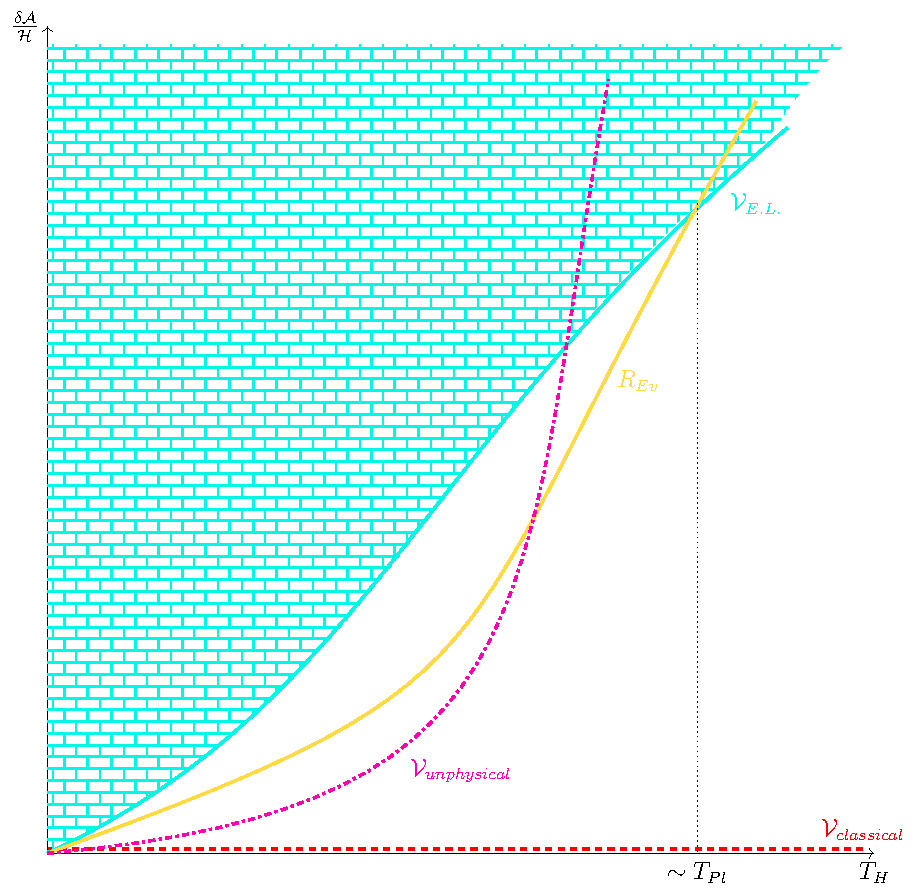
\includegraphics[scale=0.62]{Immagini/state-independent-bounds-slides/state-independent-bounds.pdf}

			\column{0.38\textwidth}
			\centering
			\vskip -15pt
			\begin{ideablock}{SNEC bound}
				\[
				\mathcal{V}_{E.L.}\Big\vert_{SNEC} \propto T_H^2	
				\]
			\end{ideablock}
			\vskip 5pt
			\(T_{cross} \sim 3\sqrt{B}\cdot 10^3 T_{Pl}\).
			Evaporation is allowed for theories sufficiently non classical.
		\end{columns}
	\end{frame}

	
	\section{Further developments}
	\begin{frame}
		\frametitle{What we would like to do next}
		\textbf{Summary}
		\begin{itemize}
			\item There is a tension between the classical Area theorem and Black Hole evaporation.
			\item The theorem we developed can in principle allow Black Hole evaporation.
			\item When tested under specific energy conditions the bound we derived agrees with the expected evaporation rate.
		\end{itemize}
		\textbf{Future prospectives}
		\begin{itemize}
			\item Test the robustness of our results by generalizing some ansatzs.
			\item Apply to other energy conditions attracting increasing interest, as dSNEC.
			\item Understanding what relations these results develop with Black Hole thermodynamics.
		\end{itemize}
	\end{frame}

	\begin{frame}[allowframebreaks]
		\frametitle{Acknowledgments}
		{\Huge
		\textcolor{turquoise!80!black}{Thank you for your attention!}}
		\vskip 15 pt
		\textbf{Selected Bibliography}
		\vskip 10 pt
		\printbibliography
	\end{frame}

\end{document}


	
	
	
	
	
	

	
	
	
	
	



